%ब 
\section{Delete} \label{s:results-Delete}

The \texttt{delete} operation triggers referential integrity validations
whenever entities are deleted.
Figure~\ref{fres:Delete} presents the results of the \texttt{delete} operation
on each entity for all the solutions.
Specifically, Figure~\ref{fres:Delete-responsetime} shows the average
response time to perform a single \texttt{delete} on each entity according to
each solution and Figure~\ref{fres:Delete-throughput} presents the
respective throughput for this operation.

	\begin{figure}[H] 
	\newcommand{\W}{.5\textwidth}
		\subfigure[Response time for Update operation]
		{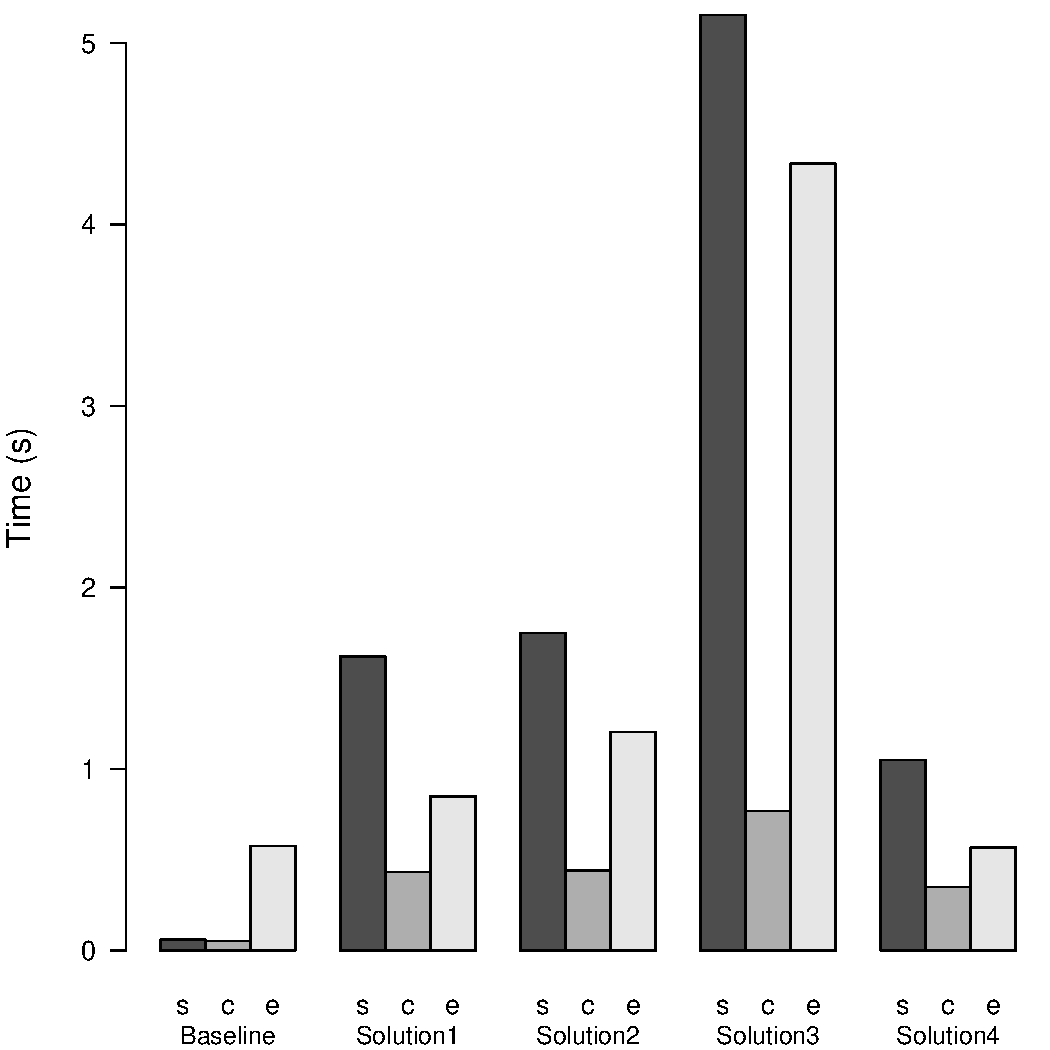
\includegraphics[width=\W]{figure/result/barplot-delete-rt.pdf} \label{fres:delete-}\label{fres:Delete-responsetime}}
		\subfigure[Throughput for Update operation]
		{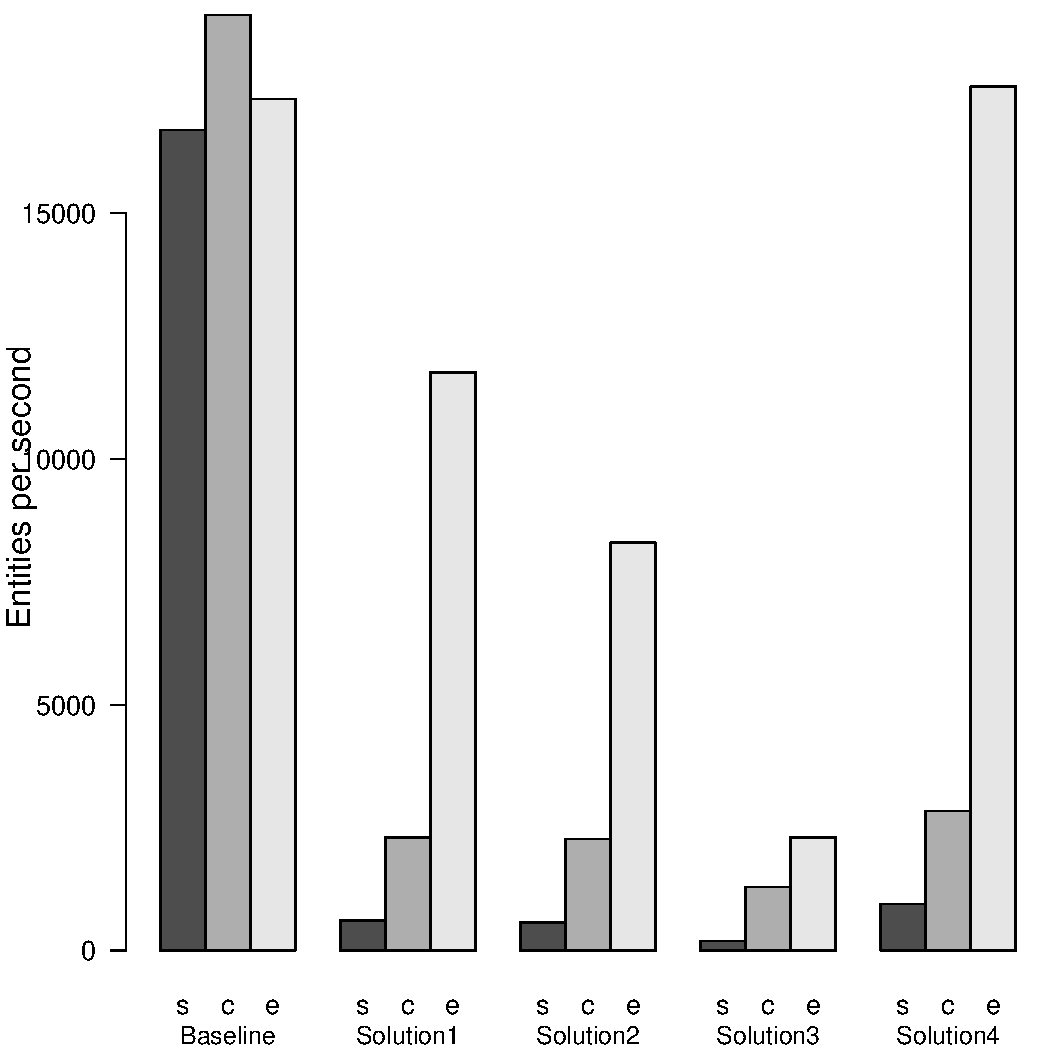
\includegraphics[width=\W]{figure/result/barplot-delete-tp.pdf} \label{fres:delete-}\label{fres:Delete-throughput}}
		\caption{Performance of Solutions in Update}\label{fres:Delete}
	\end{figure}
 
The results show that the \texttt{delete} operation on \texttt{Enrolment}
is the fastest in all the solutions. Deleting \texttt{Enrolment} entities is
faster as these have no referential integrity constraints to satisfy since
\texttt{Enrolment} has no child dependencies in it.
Nonetheless, this operation is  slower than the baseline in all the solutions
because it involves accessing metadata to retrieve the relevant constraints of
\texttt{Enrolment} in order to determine if any child dependencies exist or
not.

The \texttt{delete} operation on \texttt{Student} is the slowest. Deleting
\texttt{Student} entities is a cascaded operation which involves deleting the
child entities in the \texttt{Enrolment} column family. This operation is the
slowest because  the  child entities in \texttt{Enrolment}  which have a
reference to  \texttt{Student} have to be deleted first.

Finally, the \texttt{delete} operation on \texttt{Course} is faster than
deleting \texttt{Student} entities. Deleting \texttt{Course} entities also
involves accessing the relevant constraints and finding the child dependencies
in \texttt{Enrolment}. However, at this stage,  all the entities in
\texttt{Enrolment} are already deleted before \texttt{delete} is invoked on
\texttt{Course} entities. Hence, \texttt{delete} in \texttt{Course} actually
deletes the entities as there are no existing child dependencies.

% Notice that \texttt{delete} on \texttt{Course} involves the time to access
% metadata as well as \texttt{Enrolment} in order to search for any existing child
% dependencies and values are deleted from a single column family. However,
% \texttt{delete} on \texttt{Student} entities involve deleting values from two
% column families (\texttt{Student} and \texttt{Enrolment}). This makes
% \texttt{delete} in \texttt{Course} faster than \texttt{delete} in
% \texttt{Student}.

% As seen in \texttt{update}, the difference in  performance of the operation
% on the different entities is because of the referential integrity rules on
% child and parent entities. 





More detailed inforation about the performance of this operation can be seen in
Figures~\ref{fres:delete-response-time} and~\ref{fres:delete-throughput}.
It can be seen from these results that Solution~4 takes the least time to
complete a \texttt{delete} operation on each entity, while Solution~3 takes the
most time. Since Solution~4 caches the metadata of all the entities, it avoids
multiple accesses to the \texttt{Metadata} column family, whereas Solution~3
requires accessing \texttt{Metadata} each time a constraint has to be accessed
for an entity. The performance of Solutions~1 and 2 are comparable to each other
even though Solution~2 takes slightly more time due to its additional search
operation to locate the top row.



When compared to the baseline, all the solutions take longer to delete entities.
As mentioned previously, this is because all the solutions involve accessing
relevant constraints and performing referential integrity validations. In this
operation, when entities have child dependencies (\texttt{Student} and
\texttt{Course}), Solutions~1 and 2 are more than 23 times slower than the
baseline, Solution~3 almost 80 times slower and Solution~4   up to 17 times
slower than the baseline. On the other hand, deletes on child entities make
Solutions~1 and 2  almost 2 times slower than baseline, Solution~3  almost 7
times slower ,while Solution~4 is almost similar to the baseline, which shows
that accessing the metadata does not cause much difference in the performance.


\begin{landscape}
		\begin{figure}
		\centering
		\newcommand{\W}{.4\textwidth}
			\subfigure[Delete on Student]
			{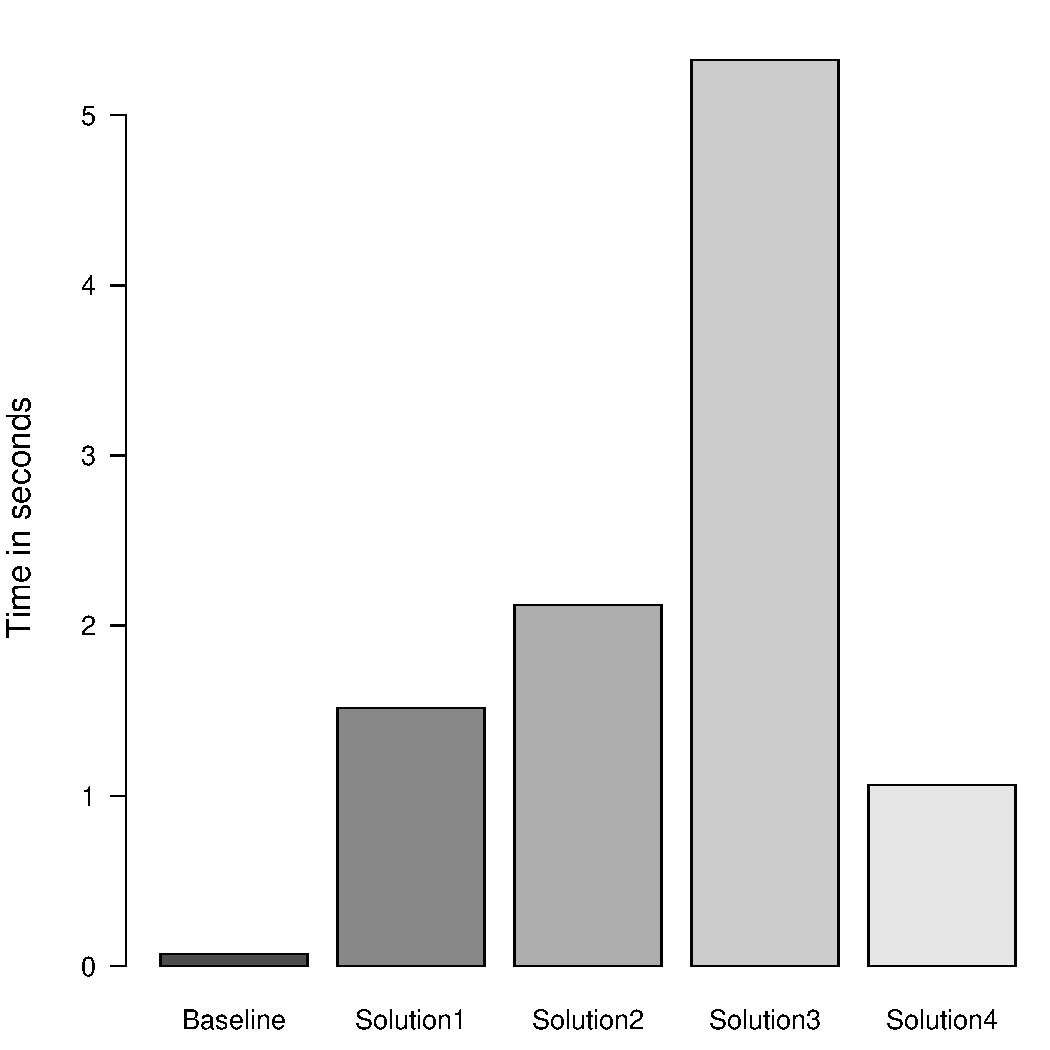
\includegraphics[width=\W]{figure/result/barplot-delete_student-rt.pdf}
			\label{fres:delete-user}}
			\subfigure[Delete on Course]
			{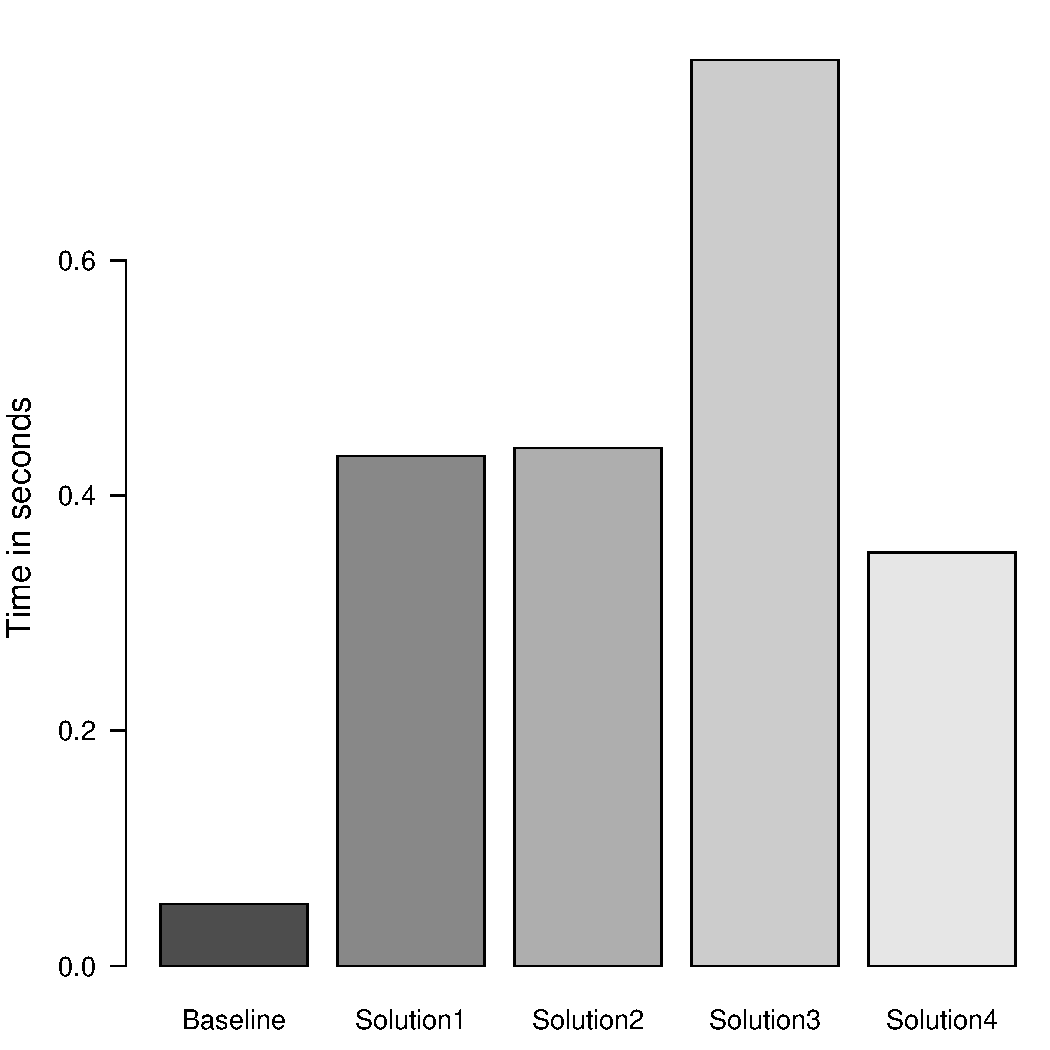
\includegraphics[width=\W]{figure/result/barplot-delete_course-rt.pdf}
			\label{fres:delete-course}}
			\subfigure[ Delete on Enrolment ]
			{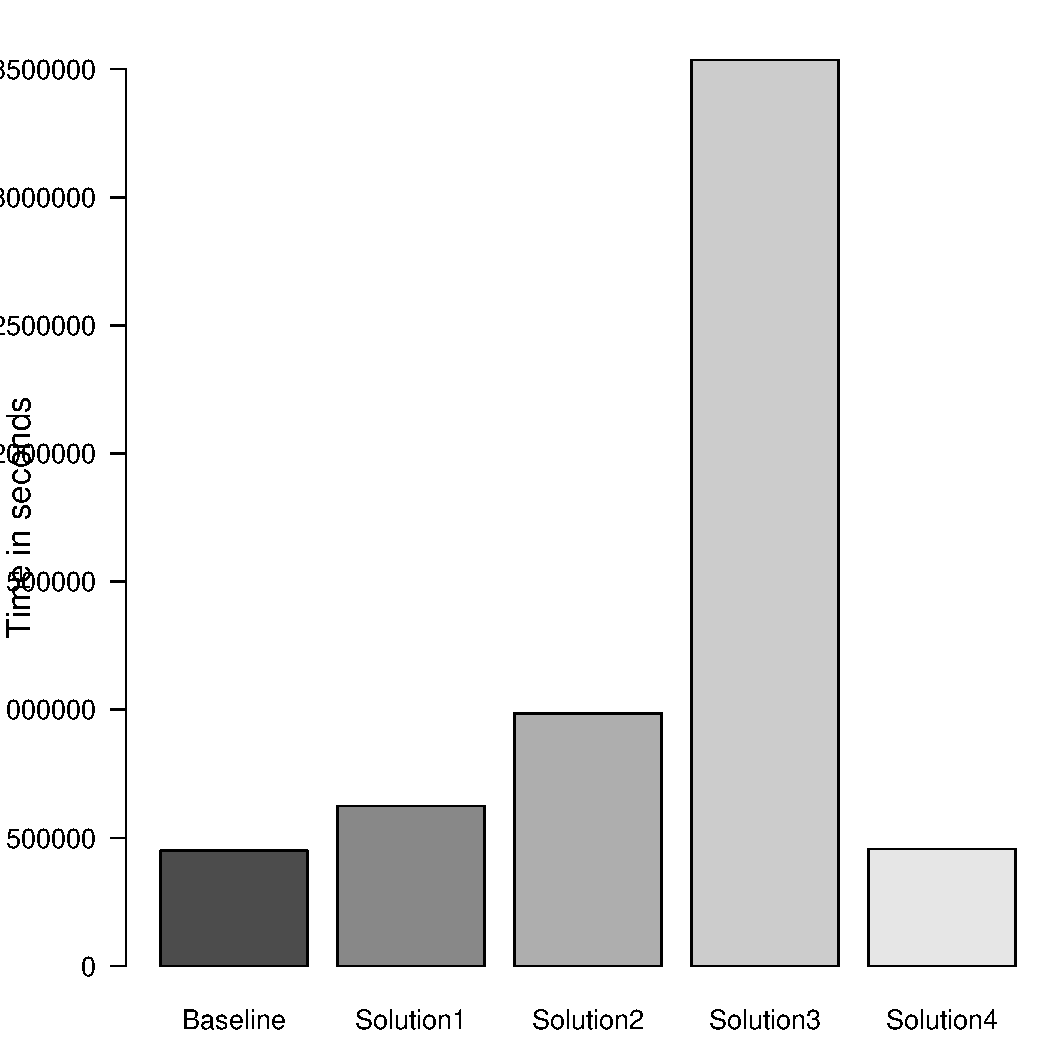
\includegraphics[width=\W]{figure/result/barplot-delete_enrolment-rt.pdf}
			\label{fres:delete-enrolment}}
			\caption{Response time deleting entities}\label{fres:delete-response-time}
						
			\subfigure[Delete on Student]
			{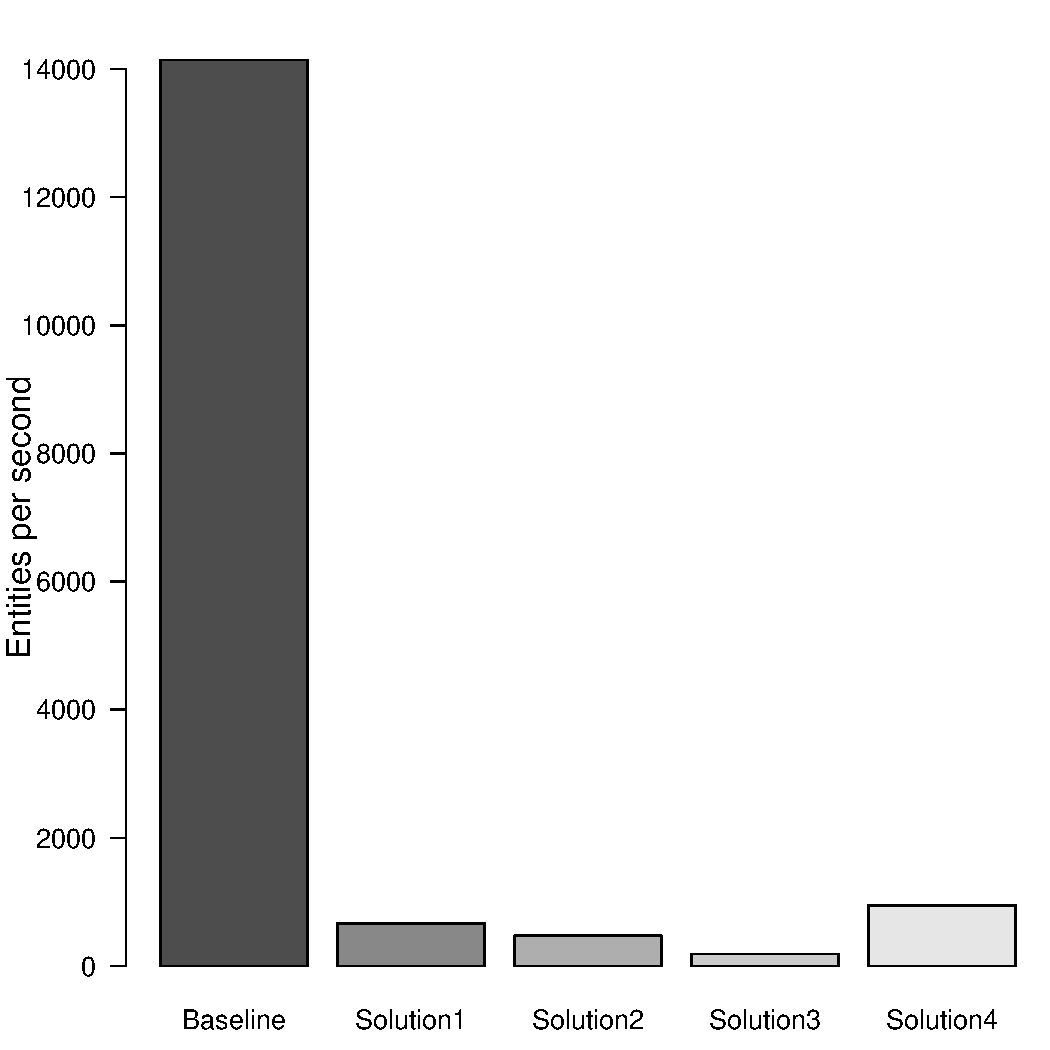
\includegraphics[width=\W]{figure/result/barplot-delete_student-tp.pdf} \label{fres:delete-}}
			\subfigure[Delete on Course]
			{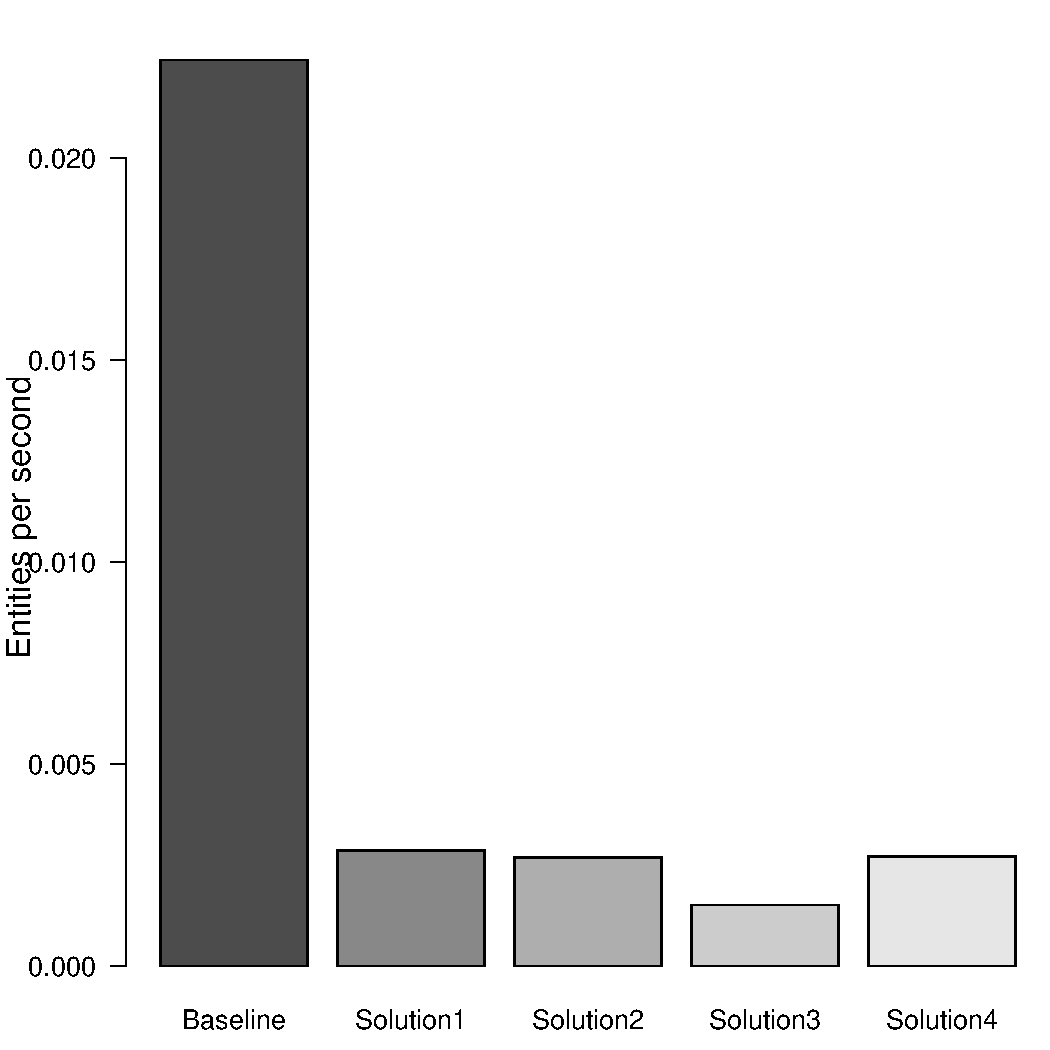
\includegraphics[width=\W]{figure/result/barplot-delete_course-tp.pdf} \label{fres:delete-}}
			\subfigure[Delete on Enrolment]
			{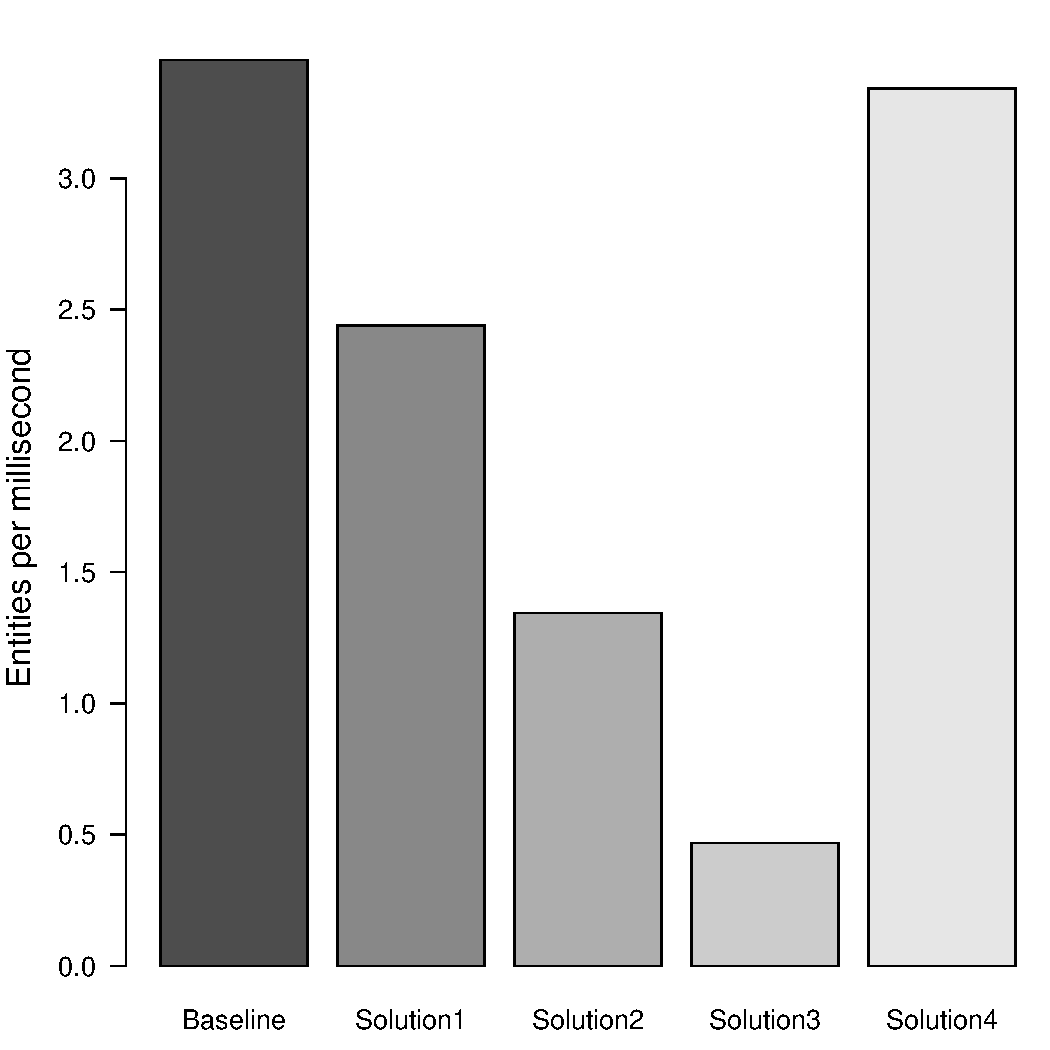
\includegraphics[width=\W]{figure/result/barplot-delete_enrolment-tp.pdf} \label{fres:delete-}}
			\caption{Throughput deleting entities}\label{fres:delete-throughput}
		\end{figure}
\end{landscape}
